\documentclass[12pt,]{article}
\usepackage{lmodern}
\usepackage{amssymb,amsmath}
\usepackage{ifxetex,ifluatex}
\usepackage{fixltx2e} % provides \textsubscript
\ifnum 0\ifxetex 1\fi\ifluatex 1\fi=0 % if pdftex
  \usepackage[T1]{fontenc}
  \usepackage[utf8]{inputenc}
\else % if luatex or xelatex
  \ifxetex
    \usepackage{mathspec}
  \else
    \usepackage{fontspec}
  \fi
  \defaultfontfeatures{Ligatures=TeX,Scale=MatchLowercase}
    \setmainfont[]{Times New Roman}
\fi
% use upquote if available, for straight quotes in verbatim environments
\IfFileExists{upquote.sty}{\usepackage{upquote}}{}
% use microtype if available
\IfFileExists{microtype.sty}{%
\usepackage{microtype}
\UseMicrotypeSet[protrusion]{basicmath} % disable protrusion for tt fonts
}{}
\usepackage[margin=2.54cm]{geometry}
\usepackage{hyperref}
\hypersetup{unicode=true,
            pdftitle={Applying Urinary Biomarkers of 11-dehydrothromboxane B2 and 8-isoprostane to Understand the Health Effects of NO2 Exposure},
            pdfauthor={Yang Wang},
            pdfborder={0 0 0},
            breaklinks=true}
\urlstyle{same}  % don't use monospace font for urls
\usepackage{color}
\usepackage{fancyvrb}
\newcommand{\VerbBar}{|}
\newcommand{\VERB}{\Verb[commandchars=\\\{\}]}
\DefineVerbatimEnvironment{Highlighting}{Verbatim}{commandchars=\\\{\}}
% Add ',fontsize=\small' for more characters per line
\usepackage{framed}
\definecolor{shadecolor}{RGB}{248,248,248}
\newenvironment{Shaded}{\begin{snugshade}}{\end{snugshade}}
\newcommand{\AlertTok}[1]{\textcolor[rgb]{0.94,0.16,0.16}{#1}}
\newcommand{\AnnotationTok}[1]{\textcolor[rgb]{0.56,0.35,0.01}{\textbf{\textit{#1}}}}
\newcommand{\AttributeTok}[1]{\textcolor[rgb]{0.77,0.63,0.00}{#1}}
\newcommand{\BaseNTok}[1]{\textcolor[rgb]{0.00,0.00,0.81}{#1}}
\newcommand{\BuiltInTok}[1]{#1}
\newcommand{\CharTok}[1]{\textcolor[rgb]{0.31,0.60,0.02}{#1}}
\newcommand{\CommentTok}[1]{\textcolor[rgb]{0.56,0.35,0.01}{\textit{#1}}}
\newcommand{\CommentVarTok}[1]{\textcolor[rgb]{0.56,0.35,0.01}{\textbf{\textit{#1}}}}
\newcommand{\ConstantTok}[1]{\textcolor[rgb]{0.00,0.00,0.00}{#1}}
\newcommand{\ControlFlowTok}[1]{\textcolor[rgb]{0.13,0.29,0.53}{\textbf{#1}}}
\newcommand{\DataTypeTok}[1]{\textcolor[rgb]{0.13,0.29,0.53}{#1}}
\newcommand{\DecValTok}[1]{\textcolor[rgb]{0.00,0.00,0.81}{#1}}
\newcommand{\DocumentationTok}[1]{\textcolor[rgb]{0.56,0.35,0.01}{\textbf{\textit{#1}}}}
\newcommand{\ErrorTok}[1]{\textcolor[rgb]{0.64,0.00,0.00}{\textbf{#1}}}
\newcommand{\ExtensionTok}[1]{#1}
\newcommand{\FloatTok}[1]{\textcolor[rgb]{0.00,0.00,0.81}{#1}}
\newcommand{\FunctionTok}[1]{\textcolor[rgb]{0.00,0.00,0.00}{#1}}
\newcommand{\ImportTok}[1]{#1}
\newcommand{\InformationTok}[1]{\textcolor[rgb]{0.56,0.35,0.01}{\textbf{\textit{#1}}}}
\newcommand{\KeywordTok}[1]{\textcolor[rgb]{0.13,0.29,0.53}{\textbf{#1}}}
\newcommand{\NormalTok}[1]{#1}
\newcommand{\OperatorTok}[1]{\textcolor[rgb]{0.81,0.36,0.00}{\textbf{#1}}}
\newcommand{\OtherTok}[1]{\textcolor[rgb]{0.56,0.35,0.01}{#1}}
\newcommand{\PreprocessorTok}[1]{\textcolor[rgb]{0.56,0.35,0.01}{\textit{#1}}}
\newcommand{\RegionMarkerTok}[1]{#1}
\newcommand{\SpecialCharTok}[1]{\textcolor[rgb]{0.00,0.00,0.00}{#1}}
\newcommand{\SpecialStringTok}[1]{\textcolor[rgb]{0.31,0.60,0.02}{#1}}
\newcommand{\StringTok}[1]{\textcolor[rgb]{0.31,0.60,0.02}{#1}}
\newcommand{\VariableTok}[1]{\textcolor[rgb]{0.00,0.00,0.00}{#1}}
\newcommand{\VerbatimStringTok}[1]{\textcolor[rgb]{0.31,0.60,0.02}{#1}}
\newcommand{\WarningTok}[1]{\textcolor[rgb]{0.56,0.35,0.01}{\textbf{\textit{#1}}}}
\usepackage{longtable,booktabs}
\usepackage{graphicx,grffile}
\makeatletter
\def\maxwidth{\ifdim\Gin@nat@width>\linewidth\linewidth\else\Gin@nat@width\fi}
\def\maxheight{\ifdim\Gin@nat@height>\textheight\textheight\else\Gin@nat@height\fi}
\makeatother
% Scale images if necessary, so that they will not overflow the page
% margins by default, and it is still possible to overwrite the defaults
% using explicit options in \includegraphics[width, height, ...]{}
\setkeys{Gin}{width=\maxwidth,height=\maxheight,keepaspectratio}
\IfFileExists{parskip.sty}{%
\usepackage{parskip}
}{% else
\setlength{\parindent}{0pt}
\setlength{\parskip}{6pt plus 2pt minus 1pt}
}
\setlength{\emergencystretch}{3em}  % prevent overfull lines
\providecommand{\tightlist}{%
  \setlength{\itemsep}{0pt}\setlength{\parskip}{0pt}}
\setcounter{secnumdepth}{5}
% Redefines (sub)paragraphs to behave more like sections
\ifx\paragraph\undefined\else
\let\oldparagraph\paragraph
\renewcommand{\paragraph}[1]{\oldparagraph{#1}\mbox{}}
\fi
\ifx\subparagraph\undefined\else
\let\oldsubparagraph\subparagraph
\renewcommand{\subparagraph}[1]{\oldsubparagraph{#1}\mbox{}}
\fi

%%% Use protect on footnotes to avoid problems with footnotes in titles
\let\rmarkdownfootnote\footnote%
\def\footnote{\protect\rmarkdownfootnote}

%%% Change title format to be more compact
\usepackage{titling}

% Create subtitle command for use in maketitle
\providecommand{\subtitle}[1]{
  \posttitle{
    \begin{center}\large#1\end{center}
    }
}

\setlength{\droptitle}{-2em}

  \title{Applying Urinary Biomarkers of 11-dehydrothromboxane B2 and
8-isoprostane to Understand the Health Effects of NO2 Exposure}
    \pretitle{\vspace{\droptitle}\centering\huge}
  \posttitle{\par}
  \subtitle{\url{https://github.com/Yang190809/data_repository_yang}}
  \author{Yang Wang}
    \preauthor{\centering\large\emph}
  \postauthor{\par}
    \date{}
    \predate{}\postdate{}
  

\begin{document}
\maketitle

\textbf{Abstract}

Mounting evidence shows that exposure to NO2 generates oxidative stress.
Oxidative stress can cause lipid damage, which plays an important role
in various respiratory and cardiovascular diseases. Urinary
8-isoprostane is a product of lipid peroxidation which can reflect
systemic lipid damage. I built linear mix models to analyze the
relationship between the level of urinary 8-isoprostane with the level
of NO2 exposure. I found that short term NO2 exposure was associated
with lipid peroxidation, reflected by increased concentrations of
urinary 8-isoprostane associated with increasing exposure. One IQR (7.41
µg/m3) incremental change of 12-h NO2 exposure was associated with an
increase of 8-isoprostane level by 19.45\% (95\% Cl: 14.37\%, 24.55\%,
p-value \textless0.001). One IQR (8.64 µg/m3) incremental change of 24-h
NO2 exposure was associated an increase in 8-isoprostane level by
27.69\% (95\% Cl: 20.50\%, 34.95\% , p-value \textless0.001). One IQR
(4.47 µg/m3) incremental change of 1-week NO2 exposure was associated
with an increase in 8-isoprostane level by 25.15\% (95\% Cl:
14.14\%,36.31\%, p-value \textless0.05). One IQR (2.74 µg/m3)
incremental change of 2-week NO2 exposure was associated with an
increase in 8-isoprostane level by 15.68\% (95\% Cl: 8.87\%,22.65\%,
p-value \textless0.05).

\newpage
\tableofcontents

\newpage

\hypertarget{rationale-and-research-questions}{%
\section{Rationale and Research
Questions}\label{rationale-and-research-questions}}

Exposure to NO2 associated with cardiovascular disease, lung function
impairment and asthma (Mölter, A., et. al.,2013, Collart, P., et.
al.,2018, Takenoue, Y., et. al., 2012 ). Mounting evidence shows that
exposure to NO2 generates oxidative stress (Hashemzadeh, B., et.
al.,2019). Oxidative stress can cause lipid damage (Black, C. N., et.
al., 2017), which plays an important role in various respiratory and
cardiovascular diseases. (Zanolin, M. E., et. a.,2015, Lakshmi, S. V.,
et. al., 2009). I applied 8-isoprostane to investigate the health
effects of short term NO2 exposure.

8-isoprostane is the product of the oxidized cell membrane after being
attacked by reactive oxygen species such as peroxides. Therefore,
8-isoprostane can reflect lipid damage (Danielsen et al., 2009).
8-isoprostane in urine does not have a diurnal variation and has been
proven to be a stable biomarker showing systemic lipid damage. It has
been applied in studying diseases such as type 2 diabetes mellitus,
obesity, coronary heart disease, asthma, and acute respiratory distress
syndrome (Nuernberg, A. M., et al., 2008). Nevertheless, the use of this
biomarker in the research of air pollution and its health effects is
scarce. One study in Iran discovered a significant positive relationship
between short-term NO2 exposure and 8-isoprostane in exhaled breath
condensate (EBC) in healthy children aged 12-13 years old (Hashemzadeh,
B., et. al., 2019). One study in New York City found that the increases
in 1- to 5-day averages of nitrogen dioxide were significantly
associated with increases in 8-isoprostane in EBC among 18-year old
healthy and asthma affected individuals (Patel, M. M., et. al., 2013).
My research question is: If the NO2 exposure is positively associated
with urinary 8-isoprostane? Among periods of 12-hour,24-hour,1-week and
2-weeks, which period has the most significant association with urinary
8-isoprostane?

\hypertarget{dataset-information}{%
\section{Dataset Information}\label{dataset-information}}

All the data are obtained from Jim Zhang's lab. The urine samples were
collected from participants of a previously described study conducted in
Changsha, China by Dr.~Zhang and other researchers ( Day, D. B., et.
al.,2018). The study recruited 89 healthy individuals
(age\textgreater18years old) who were living and working at the Broad
Company Campus and divided them into 2 groups, Group A (n = 36) and
Group B (n = 53). The study periods include pre-intervention,
intervention, and post-intervention, lasting 5 weeks. Urine samples were
collected from each participant once during the pre-intervention, twice
during the intervention, and once during the post-intervention. The
study measured hourly indoor and outdoor concentrations of PM2.5, O3,
NO2, and SO2, surveyed each participant's time-activity, and calculated
the participants' exposure for each pollutant over 12h, 24h, 1 week and
2 week periods, which were counted backward from the visit points.

The file 8-iso is the data set of urinary biomarker 8-isoprostane. The
file urine\_info is the data set that has information about the subjects
who provided the urine samples. The urine list is a data set with lists
of information of sample ID, subject ID and visits. The meaning of the
columns as well as units and class of the data in each foler is listed
below. Column names without descriptors are irrelevant to this study.

\hypertarget{urine-list-raw-data-set}{%
\subsection{Urine list raw data set}\label{urine-list-raw-data-set}}

The urine list has the information about the sample ID, subject ID and
visits.

\begin{longtable}[]{@{}llll@{}}
\toprule
Column Name & Meaning & units & class of the data\tabularnewline
\midrule
\endhead
Sample ID & the identity number of the samples & NA &
integer\tabularnewline
Subject ID & the identity number of the subjects & NA &
integer\tabularnewline
visit & the number of the 4 visits (1,2,3 or 4) & NA &
integer\tabularnewline
\bottomrule
\end{longtable}

\center \textbf{Table 1} \center 

\hypertarget{isoprostane-data-set}{%
\subsection{8-isoprostane data set}\label{isoprostane-data-set}}

The 8-isoprostane data set has information about 8-isoprostane
concentration tested in the mass spectrum and the concentration of
8-isoprostane in original urine samples. The limit of detection for
8-isoprostane was 0.016ng/ml. Any value which is below 0.016 in the
column of calculated Conc in 8-is data set should be excluded as an
error.

\begin{longtable}[]{@{}llll@{}}
\toprule
Column Name & Meaning & Units & Class of the data\tabularnewline
\midrule
\endhead
Sample ID & the identity number of the samples & NA &
integer\tabularnewline
Calculated Conc & the concentration tested by the machine & ng/ml &
numeric\tabularnewline
Sample Conc & the concentration in the original urine & ng/ml &
numeric\tabularnewline
\bottomrule
\end{longtable}

\center \textbf{Table 2} \center 

\hypertarget{urine-info}{%
\subsection{Urine Info}\label{urine-info}}

The urine info is the data set that has information about subjects
characteristics and average pollutant exposure (NO2, SO2, O3, and
PM2.5)over the periods of 12 hours, 24 hours, one week, and two weeks.
It also includes average temperature and humidity over the periods of 12
hours, 24 hours, one week, and two weeks.

\begin{longtable}[]{@{}llll@{}}
\toprule
Column name & Meaning & Units & Class of the data\tabularnewline
\midrule
\endhead
ample\_ID & the identity number of the samples & NA &
integer\tabularnewline
SubjectID & the identity number of the subjects & NA &
integer\tabularnewline
COLD & cold ( represent respiratory infection) & NA &
category\tabularnewline
MNST & menstration during visit & NA & category\tabularnewline
last.ate & the hours to the last meal & hours & integer\tabularnewline
wkday.start & the day that the subject start their work & NA &
category\tabularnewline
dt\_smoke & second-hand smoke exposure in hours & hours &
numeric\tabularnewline
USG urine & specific gravity & g/ml & numeric\tabularnewline
o3exp.12h & the exposure of ozone in 12h & ug/m3 &
numeric\tabularnewline
pmexp.12h & the exposure of PM2.5 in 12h & ug/m3 &
numeric\tabularnewline
no2exp.12h & the exposure of NO2 in 12h & ug/m3 & numeric\tabularnewline
so2exp.12h & the exposure of SO2 in 12h & ug/m3 & numeric\tabularnewline
Temp.12h & temperature in 12h & ug/m3 & numeric\tabularnewline
RHx.12h & humidity in 12h & ug/m3 & numeric\tabularnewline
\bottomrule
\end{longtable}

\center \textbf{Table 3} \center 

\hypertarget{data-wrangling}{%
\subsection{Data Wrangling}\label{data-wrangling}}

My data wrangling started with loading the data set of 8-isoprostane and
changing the column names. Then I merged this data set with the urine
list to match the sample ID with subjects ID and visit. Then this merged
data was merged with the urine info data set using the subject ID and
visit as the matching keys. After the second merging, the rows with NAs
were removed. Then I calculated the normalized 8-isoprostane using the
specific urine gravity. This normalization can adjust the dilution in
the urine. I obtained my final data by selecting columns that are
relevant to my research question. Finally, the processed data was saved
into a processed data folder.
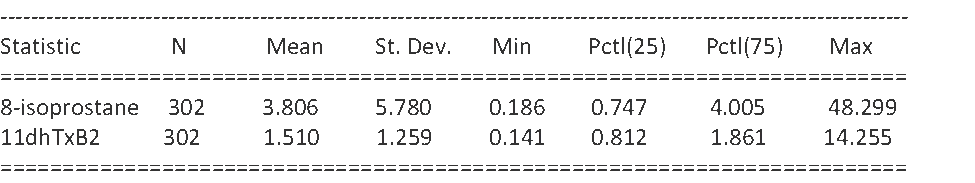
\includegraphics{C:/Users/26059/OneDrive/Desktop/ENV 872 R/Yang_ENV872/directory_yang/table.png}
\center \textbf{Table 4} \center 

\newpage

\textbf{1. Data wrangling}

\begin{Shaded}
\begin{Highlighting}[]
\CommentTok{# Set working directory}
\KeywordTok{getwd}\NormalTok{()}
\end{Highlighting}
\end{Shaded}

\begin{verbatim}
## [1] "C:/Users/26059/OneDrive/Desktop/ENV 872 R/Yang_ENV872/directory_yang"
\end{verbatim}

\begin{Shaded}
\begin{Highlighting}[]
\CommentTok{# Load packages}
\KeywordTok{library}\NormalTok{(tidyverse)}
\KeywordTok{library}\NormalTok{(lmerTest)}
\KeywordTok{library}\NormalTok{(MuMIn)}
\KeywordTok{library}\NormalTok{(car)}
\KeywordTok{library}\NormalTok{(tidyverse)}
\KeywordTok{library}\NormalTok{(cowplot)}
\KeywordTok{library}\NormalTok{(RColorBrewer)}
\CommentTok{# Set ggplot theme}
\NormalTok{mytheme <-}\StringTok{ }\KeywordTok{theme_classic}\NormalTok{(}\DataTypeTok{base_size =} \DecValTok{25}\NormalTok{) }\OperatorTok{+}
\StringTok{  }\KeywordTok{theme}\NormalTok{(}\DataTypeTok{axis.text =} \KeywordTok{element_text}\NormalTok{(}\DataTypeTok{color =} \StringTok{"black"}\NormalTok{), }
        \DataTypeTok{legend.position =} \StringTok{"top"}\NormalTok{)}
\KeywordTok{theme_set}\NormalTok{(mytheme)}

\CommentTok{# Load dataset 1}
\NormalTok{is <-}\StringTok{ }\KeywordTok{read.csv}\NormalTok{(}\StringTok{"raw_data/8iso.csv"}\NormalTok{)}
\NormalTok{is <-}\StringTok{ }\KeywordTok{select}\NormalTok{(is, Sample.ID, Calculated.Conc, Sample.Conc)}
\KeywordTok{colnames}\NormalTok{(is)[}\KeywordTok{colnames}\NormalTok{(is) }\OperatorTok{==}\StringTok{ "Calculated.Conc"}\NormalTok{] <-}\StringTok{ "is.origin"}
\KeywordTok{colnames}\NormalTok{(is)[}\KeywordTok{colnames}\NormalTok{(is) }\OperatorTok{==}\StringTok{ "Sample.Conc"}\NormalTok{] <-}\StringTok{ "is.conc"}

\CommentTok{# Load dataset 2}
\NormalTok{list <-}\StringTok{ }\KeywordTok{read.csv}\NormalTok{(}\StringTok{"raw_data/urine_list.csv"}\NormalTok{)}

\CommentTok{#merge}
\NormalTok{merge1 <-}\StringTok{ }\KeywordTok{merge}\NormalTok{(}\DataTypeTok{x=}\NormalTok{is,}\DataTypeTok{y=}\NormalTok{list,}\DataTypeTok{by=}\StringTok{"Sample.ID"}\NormalTok{,}\DataTypeTok{all=}\OtherTok{TRUE}\NormalTok{)}

\NormalTok{urine.info <-}\StringTok{ }\KeywordTok{read.csv}\NormalTok{(}\StringTok{"raw_data/urine_info.csv"}\NormalTok{)}
\NormalTok{merge3 <-}\StringTok{ }\KeywordTok{merge}\NormalTok{(}\DataTypeTok{x=}\NormalTok{merge1,}\DataTypeTok{y=}\NormalTok{urine.info,}\DataTypeTok{by=}\KeywordTok{c}\NormalTok{(}\StringTok{"Subject.ID"}\NormalTok{,}\StringTok{"visit"}\NormalTok{),}\DataTypeTok{all=}\OtherTok{TRUE}\NormalTok{)}
\KeywordTok{dim}\NormalTok{(merge3)}
\end{Highlighting}
\end{Shaded}

\begin{verbatim}
## [1] 344  69
\end{verbatim}

\begin{Shaded}
\begin{Highlighting}[]
\NormalTok{full.data <-}\StringTok{ }\KeywordTok{na.omit}\NormalTok{(merge3)}
\KeywordTok{dim}\NormalTok{(full.data)}
\end{Highlighting}
\end{Shaded}

\begin{verbatim}
## [1] 307  69
\end{verbatim}

\begin{Shaded}
\begin{Highlighting}[]
\NormalTok{mean.cre<-}\StringTok{ }\KeywordTok{mean}\NormalTok{(full.data}\OperatorTok{$}\NormalTok{USG)}
\NormalTok{mean.cre}
\end{Highlighting}
\end{Shaded}

\begin{verbatim}
## [1] 1.016117
\end{verbatim}

\begin{Shaded}
\begin{Highlighting}[]
\CommentTok{#calculate normalized biomarker concentration}
\NormalTok{full.data}\OperatorTok{$}\NormalTok{is.ad <-}\StringTok{ }\NormalTok{(full.data}\OperatorTok{$}\NormalTok{is.conc}\OperatorTok{/}\NormalTok{(}\DecValTok{1}\OperatorTok{-}\NormalTok{full.data}\OperatorTok{$}\NormalTok{USG))}\OperatorTok{*}\NormalTok{(}\DecValTok{1}\OperatorTok{-}\NormalTok{mean.cre)}

\CommentTok{#select useful colums}
\NormalTok{final.dat<-}\StringTok{ }\KeywordTok{select}\NormalTok{(full.data, Sample.ID, Subject.ID, is.ad, is.conc, is.origin, group,  COLD,   MNST,   last.ate,   wkday.start,go.home,Smoker,go.home, dt_smoke,   o3exp}\FloatTok{.12}\NormalTok{h,  pmexp}\FloatTok{.12}\NormalTok{h,no2exp}\FloatTok{.12}\NormalTok{h,   so2exp}\FloatTok{.12}\NormalTok{h, Temp}\FloatTok{.12}\NormalTok{h,   RHx}\FloatTok{.12}\NormalTok{h,    o3exp}\FloatTok{.24}\NormalTok{h,  pmexp}\FloatTok{.24}\NormalTok{h,  no2exp}\FloatTok{.24}\NormalTok{h, so2exp}\FloatTok{.24}\NormalTok{h, Temp}\FloatTok{.24}\NormalTok{h,   RHx}\FloatTok{.24}\NormalTok{h,    o3exp}\FloatTok{.1}\NormalTok{w,   pmexp}\FloatTok{.1}\NormalTok{w,   no2exp}\FloatTok{.1}\NormalTok{w,  so2exp}\FloatTok{.1}\NormalTok{w,  Temp}\FloatTok{.1}\NormalTok{w,    RHx}\FloatTok{.1}\NormalTok{w, o3exp}\FloatTok{.2}\NormalTok{w,   pmexp}\FloatTok{.2}\NormalTok{w,   no2exp}\FloatTok{.2}\NormalTok{w,  so2exp}\FloatTok{.2}\NormalTok{w,  Temp}\FloatTok{.2}\NormalTok{w,    RHx}\FloatTok{.2}\NormalTok{w )}

\CommentTok{#save processed data set}
\KeywordTok{write.csv}\NormalTok{(final.dat, }\DataTypeTok{row.names =} \OtherTok{FALSE}\NormalTok{, }\DataTypeTok{file =} \StringTok{"processed_data/final.dat.csv"}\NormalTok{)}
\end{Highlighting}
\end{Shaded}

\textbf{2.Explore the data}

\begin{Shaded}
\begin{Highlighting}[]
\KeywordTok{library}\NormalTok{(ggplot2)}
\CommentTok{#load processed data set}
\NormalTok{dat <-}\StringTok{ }\KeywordTok{read.csv}\NormalTok{(}\StringTok{"processed_data/final.dat.csv"}\NormalTok{)}
\CommentTok{#remove outliers}
\KeywordTok{summary}\NormalTok{(dat}\OperatorTok{$}\NormalTok{is.origin)}
\end{Highlighting}
\end{Shaded}

\begin{verbatim}
##    Min. 1st Qu.  Median    Mean 3rd Qu.    Max. 
##   1.508   6.220  13.421  45.703  38.281 605.614
\end{verbatim}

\begin{Shaded}
\begin{Highlighting}[]
\NormalTok{dat1<-}\StringTok{ }\NormalTok{dat[}\OperatorTok{-}\KeywordTok{c}\NormalTok{(}\DecValTok{4}\NormalTok{,}\DecValTok{7}\NormalTok{,}\DecValTok{89}\NormalTok{,}\DecValTok{147}\NormalTok{,}\DecValTok{167}\NormalTok{),]}

\CommentTok{#test normality}
\KeywordTok{shapiro.test}\NormalTok{(dat1}\OperatorTok{$}\NormalTok{is.ad)}
\end{Highlighting}
\end{Shaded}

\begin{verbatim}
## 
##  Shapiro-Wilk normality test
## 
## data:  dat1$is.ad
## W = 0.58916, p-value < 2.2e-16
\end{verbatim}

\begin{Shaded}
\begin{Highlighting}[]
\KeywordTok{shapiro.test}\NormalTok{(}\KeywordTok{log}\NormalTok{(dat1}\OperatorTok{$}\NormalTok{is.ad))}
\end{Highlighting}
\end{Shaded}

\begin{verbatim}
## 
##  Shapiro-Wilk normality test
## 
## data:  log(dat1$is.ad)
## W = 0.98127, p-value = 0.0005511
\end{verbatim}

\begin{Shaded}
\begin{Highlighting}[]
\CommentTok{#explore the data}

\CommentTok{#calculate IQR for each period}
\NormalTok{sum3<-}\KeywordTok{summary}\NormalTok{(dat}\OperatorTok{$}\NormalTok{no2exp}\FloatTok{.12}\NormalTok{h)}
\NormalTok{no2}\FloatTok{.12}\NormalTok{ <-sum3[}\DecValTok{5}\NormalTok{]}\OperatorTok{-}\NormalTok{sum3[}\DecValTok{2}\NormalTok{]}
\NormalTok{no2}\FloatTok{.12}
\end{Highlighting}
\end{Shaded}

\begin{verbatim}
##  3rd Qu. 
## 7.409404
\end{verbatim}

\begin{Shaded}
\begin{Highlighting}[]
\NormalTok{sum4<-}\KeywordTok{summary}\NormalTok{(dat}\OperatorTok{$}\NormalTok{no2exp}\FloatTok{.24}\NormalTok{h)}
\NormalTok{no2}\FloatTok{.24}\NormalTok{ <-sum4[}\DecValTok{5}\NormalTok{]}\OperatorTok{-}\NormalTok{sum4[}\DecValTok{2}\NormalTok{]}
\NormalTok{no2}\FloatTok{.24}
\end{Highlighting}
\end{Shaded}

\begin{verbatim}
##  3rd Qu. 
## 8.638027
\end{verbatim}

\begin{Shaded}
\begin{Highlighting}[]
\NormalTok{sum5<-}\KeywordTok{summary}\NormalTok{(dat}\OperatorTok{$}\NormalTok{no2exp}\FloatTok{.1}\NormalTok{w)}
\NormalTok{no2}\FloatTok{.1}\NormalTok{w <-sum5[}\DecValTok{5}\NormalTok{]}\OperatorTok{-}\NormalTok{sum5[}\DecValTok{2}\NormalTok{]}
\NormalTok{no2}\FloatTok{.1}\NormalTok{w}
\end{Highlighting}
\end{Shaded}

\begin{verbatim}
##  3rd Qu. 
## 8.617326
\end{verbatim}

\begin{Shaded}
\begin{Highlighting}[]
\NormalTok{sum6<-}\KeywordTok{summary}\NormalTok{(dat}\OperatorTok{$}\NormalTok{no2exp}\FloatTok{.2}\NormalTok{w)}
\NormalTok{no2}\FloatTok{.2}\NormalTok{w <-sum6[}\DecValTok{5}\NormalTok{]}\OperatorTok{-}\NormalTok{sum6[}\DecValTok{2}\NormalTok{]}
\NormalTok{no2}\FloatTok{.2}\NormalTok{w}
\end{Highlighting}
\end{Shaded}

\begin{verbatim}
##  3rd Qu. 
## 2.736119
\end{verbatim}

\textbf{3.Build models}

3.1 Build models for 12-hour NO2 exposure

\begin{Shaded}
\begin{Highlighting}[]
\NormalTok{mo1<-}\StringTok{ }\KeywordTok{lmer}\NormalTok{(}\KeywordTok{log}\NormalTok{(is.ad) }\OperatorTok{~}\NormalTok{no2exp}\FloatTok{.12}\NormalTok{h}\OperatorTok{+}\NormalTok{o3exp}\FloatTok{.12}\NormalTok{h}\OperatorTok{+}\StringTok{ }\NormalTok{pmexp}\FloatTok{.12}\NormalTok{h}\OperatorTok{+}\NormalTok{so2exp}\FloatTok{.12}\NormalTok{h}\OperatorTok{+}\NormalTok{Temp}\FloatTok{.12}\NormalTok{h}\OperatorTok{+}\NormalTok{RHx}\FloatTok{.12}\NormalTok{h }\OperatorTok{+}\StringTok{ }\NormalTok{last.ate }\OperatorTok{+}\NormalTok{wkday.start}\OperatorTok{+}\NormalTok{go.home}\OperatorTok{+}\NormalTok{COLD}\OperatorTok{+}\NormalTok{MNST}\OperatorTok{+}\NormalTok{dt_smoke }\OperatorTok{+}\NormalTok{(}\DecValTok{1}\OperatorTok{|}\NormalTok{Subject.ID),}\DataTypeTok{data=}\NormalTok{dat1)}
\CommentTok{#find the best model with lowest AIC}
\KeywordTok{step}\NormalTok{(mo1)}
\end{Highlighting}
\end{Shaded}

\begin{verbatim}
## Backward reduced random-effect table:
## 
##                  Eliminated npar  logLik     AIC    LRT Df Pr(>Chisq)    
## <none>                        16 -474.63  981.26                         
## (1 | Subject.ID)          0   15 -493.94 1017.88 38.616  1  5.159e-10 ***
## ---
## Signif. codes:  0 '***' 0.001 '**' 0.01 '*' 0.05 '.' 0.1 ' ' 1
## 
## Backward reduced fixed-effect table:
## Degrees of freedom method: Satterthwaite 
## 
##             Eliminated  Sum Sq Mean Sq NumDF   DenDF F value   Pr(>F)    
## Temp.12h             1  0.0261  0.0261     1 276.301  0.0314 0.859411    
## COLD                 2  0.0677  0.0677     1 266.912  0.0819 0.774976    
## pmexp.12h            3  0.0956  0.0956     1 271.141  0.1159 0.733779    
## go.home              4  0.6585  0.3293     2  83.839  0.4012 0.670812    
## wkday.start          5  0.3986  0.3986     1 291.709  0.4848 0.486792    
## so2exp.12h           6  0.4401  0.4401     1 293.944  0.5343 0.465386    
## MNST                 7  0.8942  0.8942     1 272.520  1.0861 0.298261    
## last.ate             8  0.8829  0.8829     1 276.178  1.0773 0.300216    
## dt_smoke             9  0.9658  0.9658     1 293.061  1.1845 0.277332    
## RHx.12h             10  2.0108  2.0108     1 251.786  2.4885 0.115939    
## no2exp.12h           0 12.2057 12.2057     1 228.742 14.9910 0.000141 ***
## o3exp.12h            0  4.0334  4.0334     1 225.577  4.9538 0.027023 *  
## ---
## Signif. codes:  0 '***' 0.001 '**' 0.01 '*' 0.05 '.' 0.1 ' ' 1
## 
## Model found:
## log(is.ad) ~ no2exp.12h + o3exp.12h + (1 | Subject.ID)
\end{verbatim}

\begin{Shaded}
\begin{Highlighting}[]
\CommentTok{#best model for 12-hour NO2 exposure}
\NormalTok{mo1}\FloatTok{.1}\NormalTok{<-}\StringTok{ }\KeywordTok{lmer}\NormalTok{(}\KeywordTok{log}\NormalTok{(is.ad) }\OperatorTok{~}\StringTok{ }\NormalTok{no2exp}\FloatTok{.12}\NormalTok{h }\OperatorTok{+}\NormalTok{o3exp}\FloatTok{.12}\NormalTok{h }\OperatorTok{+}\StringTok{ }\NormalTok{(}\DecValTok{1} \OperatorTok{|}\StringTok{ }\NormalTok{Subject.ID),}\DataTypeTok{data=}\NormalTok{dat1)}
\KeywordTok{summary}\NormalTok{(mo1}\FloatTok{.1}\NormalTok{)}
\end{Highlighting}
\end{Shaded}

\begin{verbatim}
## Linear mixed model fit by REML. t-tests use Satterthwaite's method [
## lmerModLmerTest]
## Formula: log(is.ad) ~ no2exp.12h + o3exp.12h + (1 | Subject.ID)
##    Data: dat1
## 
## REML criterion at convergence: 910.8
## 
## Scaled residuals: 
##      Min       1Q   Median       3Q      Max 
## -1.99963 -0.62729 -0.03595  0.60429  2.58701 
## 
## Random effects:
##  Groups     Name        Variance Std.Dev.
##  Subject.ID (Intercept) 0.5187   0.7202  
##  Residual               0.8142   0.9023  
## Number of obs: 302, groups:  Subject.ID, 89
## 
## Fixed effects:
##               Estimate Std. Error         df t value Pr(>|t|)    
## (Intercept)  -0.187878   0.212372 292.646414  -0.885 0.377064    
## no2exp.12h    0.025912   0.006693 228.741989   3.872 0.000141 ***
## o3exp.12h     0.031066   0.013958 225.576673   2.226 0.027023 *  
## ---
## Signif. codes:  0 '***' 0.001 '**' 0.01 '*' 0.05 '.' 0.1 ' ' 1
## 
## Correlation of Fixed Effects:
##            (Intr) n2x.12
## no2exp.12h -0.812       
## o3exp.12h  -0.489  0.132
\end{verbatim}

\begin{Shaded}
\begin{Highlighting}[]
\CommentTok{#check F value}
\KeywordTok{anova}\NormalTok{(mo1}\FloatTok{.1}\NormalTok{)}
\end{Highlighting}
\end{Shaded}

\begin{verbatim}
## Type III Analysis of Variance Table with Satterthwaite's method
##             Sum Sq Mean Sq NumDF  DenDF F value   Pr(>F)    
## no2exp.12h 12.2057 12.2057     1 228.74 14.9910 0.000141 ***
## o3exp.12h   4.0334  4.0334     1 225.58  4.9538 0.027023 *  
## ---
## Signif. codes:  0 '***' 0.001 '**' 0.01 '*' 0.05 '.' 0.1 ' ' 1
\end{verbatim}

\begin{Shaded}
\begin{Highlighting}[]
\CommentTok{#check collinearirty}
\KeywordTok{vif}\NormalTok{(mo1}\FloatTok{.1}\NormalTok{)}
\end{Highlighting}
\end{Shaded}

\begin{verbatim}
## no2exp.12h  o3exp.12h 
##   1.017673   1.017673
\end{verbatim}

\begin{Shaded}
\begin{Highlighting}[]
\CommentTok{#get R^2}
\KeywordTok{r.squaredGLMM}\NormalTok{ (mo1}\FloatTok{.1}\NormalTok{)}
\end{Highlighting}
\end{Shaded}

\begin{verbatim}
##             R2m      R2c
## [1,] 0.03761012 0.412126
\end{verbatim}

\begin{Shaded}
\begin{Highlighting}[]
\CommentTok{#identify outliers}
\NormalTok{res1}\FloatTok{.1}\NormalTok{ <-}\StringTok{ }\KeywordTok{resid}\NormalTok{(mo1, }\DataTypeTok{type =} \StringTok{"pearson"}\NormalTok{)}
\NormalTok{dat[}\KeywordTok{which}\NormalTok{(}\KeywordTok{abs}\NormalTok{(res1}\FloatTok{.1}\NormalTok{) }\OperatorTok{>}\StringTok{ }\FloatTok{2.5}\NormalTok{),]}
\end{Highlighting}
\end{Shaded}

\begin{verbatim}
##  [1] Sample.ID   Subject.ID  is.ad       is.conc     is.origin   group      
##  [7] COLD        MNST        last.ate    wkday.start go.home     Smoker     
## [13] dt_smoke    o3exp.12h   pmexp.12h   no2exp.12h  so2exp.12h  Temp.12h   
## [19] RHx.12h     o3exp.24h   pmexp.24h   no2exp.24h  so2exp.24h  Temp.24h   
## [25] RHx.24h     o3exp.1w    pmexp.1w    no2exp.1w   so2exp.1w   Temp.1w    
## [31] RHx.1w      o3exp.2w    pmexp.2w    no2exp.2w   so2exp.2w   Temp.2w    
## [37] RHx.2w     
## <0 rows> (or 0-length row.names)
\end{verbatim}

\begin{Shaded}
\begin{Highlighting}[]
\CommentTok{#calculate IQR change}
\NormalTok{(}\KeywordTok{exp}\NormalTok{(}\FloatTok{0.025912}\NormalTok{)}\OperatorTok{-}\DecValTok{1}\NormalTok{)}\OperatorTok{*}\NormalTok{no2}\FloatTok{.12}
\end{Highlighting}
\end{Shaded}

\begin{verbatim}
##   3rd Qu. 
## 0.1945016
\end{verbatim}

\begin{Shaded}
\begin{Highlighting}[]
\NormalTok{(}\KeywordTok{exp}\NormalTok{(}\FloatTok{0.025912} \FloatTok{+0.006693}\NormalTok{)}\OperatorTok{-}\DecValTok{1}\NormalTok{)}\OperatorTok{*}\NormalTok{no2}\FloatTok{.12}
\end{Highlighting}
\end{Shaded}

\begin{verbatim}
##   3rd Qu. 
## 0.2455652
\end{verbatim}

\begin{Shaded}
\begin{Highlighting}[]
\NormalTok{(}\KeywordTok{exp}\NormalTok{(}\FloatTok{0.025912} \FloatTok{-0.006693}\NormalTok{)}\OperatorTok{-}\DecValTok{1}\NormalTok{)}\OperatorTok{*}\NormalTok{no2}\FloatTok{.12}
\end{Highlighting}
\end{Shaded}

\begin{verbatim}
##   3rd Qu. 
## 0.1437785
\end{verbatim}

3.2 Build models for 24-hour NO2 exposure

\begin{Shaded}
\begin{Highlighting}[]
\NormalTok{mo2<-}\StringTok{ }\KeywordTok{lmer}\NormalTok{(}\KeywordTok{log}\NormalTok{(is.ad) }\OperatorTok{~}\StringTok{ }\NormalTok{no2exp}\FloatTok{.24}\NormalTok{h}\OperatorTok{+}\NormalTok{o3exp}\FloatTok{.24}\NormalTok{h}\OperatorTok{+}\StringTok{ }\NormalTok{pmexp}\FloatTok{.24}\NormalTok{h}\OperatorTok{+}\NormalTok{so2exp}\FloatTok{.24}\NormalTok{h}\OperatorTok{+}\NormalTok{Temp}\FloatTok{.24}\NormalTok{h}\OperatorTok{+}\NormalTok{RHx}\FloatTok{.24}\NormalTok{h }\OperatorTok{+}\StringTok{ }\NormalTok{last.ate }\OperatorTok{+}\NormalTok{wkday.start}\OperatorTok{+}\NormalTok{go.home}\OperatorTok{+}\NormalTok{COLD}\OperatorTok{+}\NormalTok{MNST}\OperatorTok{+}\NormalTok{dt_smoke }\OperatorTok{+}\NormalTok{(}\DecValTok{1}\OperatorTok{|}\NormalTok{Subject.ID),}\DataTypeTok{data=}\NormalTok{dat1)}
\KeywordTok{step}\NormalTok{(mo2)}
\end{Highlighting}
\end{Shaded}

\begin{verbatim}
## Backward reduced random-effect table:
## 
##                  Eliminated npar  logLik     AIC    LRT Df Pr(>Chisq)    
## <none>                        16 -475.04  982.07                         
## (1 | Subject.ID)          0   15 -493.92 1017.84 37.768  1  7.969e-10 ***
## ---
## Signif. codes:  0 '***' 0.001 '**' 0.01 '*' 0.05 '.' 0.1 ' ' 1
## 
## Backward reduced fixed-effect table:
## Degrees of freedom method: Satterthwaite 
## 
##             Eliminated  Sum Sq Mean Sq NumDF   DenDF F value    Pr(>F)    
## so2exp.24h           1  0.0016  0.0016     1 280.151  0.0019 0.9655516    
## Temp.24h             2  0.0161  0.0161     1 277.135  0.0193 0.8895889    
## wkday.start          3  0.0126  0.0126     1 279.050  0.0152 0.9021154    
## COLD                 4  0.1555  0.1555     1 268.565  0.1873 0.6655198    
## go.home              5  0.9235  0.4617     2  84.443  0.5575 0.5747522    
## RHx.24h              6  0.4390  0.4390     1 258.415  0.5298 0.4673562    
## dt_smoke             7  0.5832  0.5832     1 291.289  0.7037 0.4022322    
## pmexp.24h            8  0.8868  0.8868     1 273.549  1.0799 0.2996466    
## MNST                 9  0.8850  0.8850     1 274.024  1.0795 0.2997231    
## last.ate            10  1.0377  1.0377     1 281.175  1.2708 0.2605860    
## no2exp.24h           0 12.3002 12.3002     1 231.652 15.1608 0.0001292 ***
## o3exp.24h            0  5.0095  5.0095     1 225.520  6.1746 0.0136869 *  
## ---
## Signif. codes:  0 '***' 0.001 '**' 0.01 '*' 0.05 '.' 0.1 ' ' 1
## 
## Model found:
## log(is.ad) ~ no2exp.24h + o3exp.24h + (1 | Subject.ID)
\end{verbatim}

\begin{Shaded}
\begin{Highlighting}[]
\NormalTok{mo2}\FloatTok{.1}\NormalTok{<-}\StringTok{ }\KeywordTok{lmer}\NormalTok{(}\KeywordTok{log}\NormalTok{(is.ad) }\OperatorTok{~}\StringTok{ }\NormalTok{no2exp}\FloatTok{.24}\NormalTok{h }\OperatorTok{+}\StringTok{ }\NormalTok{o3exp}\FloatTok{.24}\NormalTok{h }\OperatorTok{+}\StringTok{ }\NormalTok{(}\DecValTok{1} \OperatorTok{|}\StringTok{ }\NormalTok{Subject.ID),}\DataTypeTok{data=}\NormalTok{dat1)}
\KeywordTok{summary}\NormalTok{(mo2}\FloatTok{.1}\NormalTok{)}
\end{Highlighting}
\end{Shaded}

\begin{verbatim}
## Linear mixed model fit by REML. t-tests use Satterthwaite's method [
## lmerModLmerTest]
## Formula: log(is.ad) ~ no2exp.24h + o3exp.24h + (1 | Subject.ID)
##    Data: dat1
## 
## REML criterion at convergence: 910.4
## 
## Scaled residuals: 
##      Min       1Q   Median       3Q      Max 
## -1.88882 -0.65529 -0.03642  0.58790  2.66141 
## 
## Random effects:
##  Groups     Name        Variance Std.Dev.
##  Subject.ID (Intercept) 0.5243   0.7241  
##  Residual               0.8113   0.9007  
## Number of obs: 302, groups:  Subject.ID, 89
## 
## Fixed effects:
##               Estimate Std. Error         df t value Pr(>|t|)    
## (Intercept)  -0.339832   0.243838 284.149326  -1.394 0.164503    
## no2exp.24h    0.031555   0.008104 231.652052   3.894 0.000129 ***
## o3exp.24h     0.030798   0.012394 225.520144   2.485 0.013687 *  
## ---
## Signif. codes:  0 '***' 0.001 '**' 0.01 '*' 0.05 '.' 0.1 ' ' 1
## 
## Correlation of Fixed Effects:
##            (Intr) n2x.24
## no2exp.24h -0.857       
## o3exp.24h  -0.505  0.196
\end{verbatim}

\begin{Shaded}
\begin{Highlighting}[]
\KeywordTok{anova}\NormalTok{(mo2}\FloatTok{.1}\NormalTok{)}
\end{Highlighting}
\end{Shaded}

\begin{verbatim}
## Type III Analysis of Variance Table with Satterthwaite's method
##             Sum Sq Mean Sq NumDF  DenDF F value    Pr(>F)    
## no2exp.24h 12.3002 12.3002     1 231.65 15.1608 0.0001292 ***
## o3exp.24h   5.0095  5.0095     1 225.52  6.1746 0.0136869 *  
## ---
## Signif. codes:  0 '***' 0.001 '**' 0.01 '*' 0.05 '.' 0.1 ' ' 1
\end{verbatim}

\begin{Shaded}
\begin{Highlighting}[]
\KeywordTok{vif}\NormalTok{(mo2}\FloatTok{.1}\NormalTok{)}
\end{Highlighting}
\end{Shaded}

\begin{verbatim}
## no2exp.24h  o3exp.24h 
##   1.039908   1.039908
\end{verbatim}

\begin{Shaded}
\begin{Highlighting}[]
\KeywordTok{r.squaredGLMM}\NormalTok{ (mo2}\FloatTok{.1}\NormalTok{)}
\end{Highlighting}
\end{Shaded}

\begin{verbatim}
##             R2m       R2c
## [1,] 0.03854593 0.4159847
\end{verbatim}

\begin{Shaded}
\begin{Highlighting}[]
\NormalTok{res2}\FloatTok{.1}\NormalTok{ <-}\StringTok{ }\KeywordTok{resid}\NormalTok{(mo2}\FloatTok{.1}\NormalTok{, }\DataTypeTok{type =} \StringTok{"pearson"}\NormalTok{)}
\NormalTok{dat[}\KeywordTok{which}\NormalTok{(}\KeywordTok{abs}\NormalTok{(res2}\FloatTok{.1}\NormalTok{) }\OperatorTok{>}\StringTok{ }\FloatTok{2.5}\NormalTok{),]}
\end{Highlighting}
\end{Shaded}

\begin{verbatim}
##  [1] Sample.ID   Subject.ID  is.ad       is.conc     is.origin   group      
##  [7] COLD        MNST        last.ate    wkday.start go.home     Smoker     
## [13] dt_smoke    o3exp.12h   pmexp.12h   no2exp.12h  so2exp.12h  Temp.12h   
## [19] RHx.12h     o3exp.24h   pmexp.24h   no2exp.24h  so2exp.24h  Temp.24h   
## [25] RHx.24h     o3exp.1w    pmexp.1w    no2exp.1w   so2exp.1w   Temp.1w    
## [31] RHx.1w      o3exp.2w    pmexp.2w    no2exp.2w   so2exp.2w   Temp.2w    
## [37] RHx.2w     
## <0 rows> (or 0-length row.names)
\end{verbatim}

\begin{Shaded}
\begin{Highlighting}[]
\CommentTok{#calculate IQR change}
\NormalTok{(}\KeywordTok{exp}\NormalTok{(}\FloatTok{0.031555}\NormalTok{)}\OperatorTok{-}\DecValTok{1}\NormalTok{)}\OperatorTok{*}\NormalTok{no2}\FloatTok{.24}
\end{Highlighting}
\end{Shaded}

\begin{verbatim}
##  3rd Qu. 
## 0.276919
\end{verbatim}

\begin{Shaded}
\begin{Highlighting}[]
\NormalTok{(}\KeywordTok{exp}\NormalTok{(}\FloatTok{0.031555} \FloatTok{+0.008104}\NormalTok{)}\OperatorTok{-}\DecValTok{1}\NormalTok{)}\OperatorTok{*}\NormalTok{no2}\FloatTok{.24}
\end{Highlighting}
\end{Shaded}

\begin{verbatim}
##   3rd Qu. 
## 0.3494593
\end{verbatim}

\begin{Shaded}
\begin{Highlighting}[]
\NormalTok{(}\KeywordTok{exp}\NormalTok{(}\FloatTok{0.031555} \FloatTok{-0.008104}\NormalTok{)}\OperatorTok{-}\DecValTok{1}\NormalTok{)}\OperatorTok{*}\NormalTok{no2}\FloatTok{.24}
\end{Highlighting}
\end{Shaded}

\begin{verbatim}
##   3rd Qu. 
## 0.2049643
\end{verbatim}

3.3 Build models for 1-week NO2 exposure

\begin{Shaded}
\begin{Highlighting}[]
\NormalTok{mo3<-}\StringTok{ }\KeywordTok{lmer}\NormalTok{(}\KeywordTok{log}\NormalTok{(is.ad) }\OperatorTok{~}\StringTok{ }\NormalTok{no2exp}\FloatTok{.1}\NormalTok{w}\OperatorTok{+}\NormalTok{o3exp}\FloatTok{.1}\NormalTok{w}\OperatorTok{+}\StringTok{ }\NormalTok{pmexp}\FloatTok{.1}\NormalTok{w}\OperatorTok{+}\NormalTok{so2exp}\FloatTok{.1}\NormalTok{w}\OperatorTok{+}\NormalTok{Temp}\FloatTok{.1}\NormalTok{w}\OperatorTok{+}\NormalTok{RHx}\FloatTok{.1}\NormalTok{w }\OperatorTok{+}\StringTok{ }\NormalTok{last.ate }\OperatorTok{+}\NormalTok{wkday.start}\OperatorTok{+}\NormalTok{go.home}\OperatorTok{+}\NormalTok{COLD}\OperatorTok{+}\NormalTok{MNST}\OperatorTok{+}\NormalTok{dt_smoke }\OperatorTok{+}\NormalTok{(}\DecValTok{1}\OperatorTok{|}\NormalTok{Subject.ID),}\DataTypeTok{data=}\NormalTok{dat1)}
\KeywordTok{step}\NormalTok{(mo3)}
\end{Highlighting}
\end{Shaded}

\begin{verbatim}
## Backward reduced random-effect table:
## 
##                  Eliminated npar  logLik     AIC    LRT Df Pr(>Chisq)    
## <none>                        16 -475.45  982.89                         
## (1 | Subject.ID)          0   15 -493.45 1016.90 36.001  1  1.972e-09 ***
## ---
## Signif. codes:  0 '***' 0.001 '**' 0.01 '*' 0.05 '.' 0.1 ' ' 1
## 
## Backward reduced fixed-effect table:
## Degrees of freedom method: Satterthwaite 
## 
##             Eliminated Sum Sq Mean Sq NumDF   DenDF F value    Pr(>F)    
## Temp.1w              1 0.0000  0.0000     1 256.639  0.0000 0.9986105    
## RHx.1w               2 0.0271  0.0271     1 288.772  0.0317 0.8588147    
## COLD                 3 0.0560  0.0560     1 271.043  0.0657 0.7979384    
## wkday.start          4 0.1240  0.1240     1 258.909  0.1459 0.7027697    
## go.home              5 0.8717  0.4359     2  84.614  0.5134 0.6002845    
## pmexp.1w             6 0.2371  0.2371     1 293.316  0.2793 0.5975635    
## dt_smoke             7 0.4455  0.4455     1 291.942  0.5270 0.4684347    
## last.ate             8 0.6026  0.6026     1 277.597  0.7195 0.3970452    
## MNST                 9 0.7572  0.7572     1 273.657  0.9102 0.3409085    
## o3exp.1w            10 1.4655  1.4655     1 229.000  1.7684 0.1849006    
## no2exp.1w            0 4.4044  4.4044     1 229.706  5.2961 0.0222690 *  
## so2exp.1w            0 9.8969  9.8969     1 230.979 11.9006 0.0006669 ***
## ---
## Signif. codes:  0 '***' 0.001 '**' 0.01 '*' 0.05 '.' 0.1 ' ' 1
## 
## Model found:
## log(is.ad) ~ no2exp.1w + so2exp.1w + (1 | Subject.ID)
\end{verbatim}

\begin{Shaded}
\begin{Highlighting}[]
\NormalTok{mo3}\FloatTok{.1}\NormalTok{<-}\StringTok{ }\KeywordTok{lmer}\NormalTok{(}\KeywordTok{log}\NormalTok{(is.ad) }\OperatorTok{~}\StringTok{ }\NormalTok{no2exp}\FloatTok{.1}\NormalTok{w }\OperatorTok{+}\StringTok{ }\NormalTok{so2exp}\FloatTok{.1}\NormalTok{w }\OperatorTok{+}\StringTok{ }\NormalTok{(}\DecValTok{1} \OperatorTok{|}\StringTok{ }\NormalTok{Subject.ID),}\DataTypeTok{data=}\NormalTok{dat1)}
\KeywordTok{summary}\NormalTok{(mo3}\FloatTok{.1}\NormalTok{)}
\end{Highlighting}
\end{Shaded}

\begin{verbatim}
## Linear mixed model fit by REML. t-tests use Satterthwaite's method [
## lmerModLmerTest]
## Formula: log(is.ad) ~ no2exp.1w + so2exp.1w + (1 | Subject.ID)
##    Data: dat1
## 
## REML criterion at convergence: 913.2
## 
## Scaled residuals: 
##      Min       1Q   Median       3Q      Max 
## -1.95288 -0.61932 -0.07413  0.62697  2.63863 
## 
## Random effects:
##  Groups     Name        Variance Std.Dev.
##  Subject.ID (Intercept) 0.5199   0.7211  
##  Residual               0.8316   0.9119  
## Number of obs: 302, groups:  Subject.ID, 89
## 
## Fixed effects:
##              Estimate Std. Error        df t value Pr(>|t|)    
## (Intercept)   0.76276    0.29669 261.12832   2.571 0.010698 *  
## no2exp.1w     0.02877    0.01250 229.70566   2.301 0.022269 *  
## so2exp.1w    -0.12342    0.03578 230.97927  -3.450 0.000667 ***
## ---
## Signif. codes:  0 '***' 0.001 '**' 0.01 '*' 0.05 '.' 0.1 ' ' 1
## 
## Correlation of Fixed Effects:
##           (Intr) n2xp.1
## no2exp.1w -0.624       
## so2exp.1w -0.331 -0.476
\end{verbatim}

\begin{Shaded}
\begin{Highlighting}[]
\KeywordTok{anova}\NormalTok{(mo3}\FloatTok{.1}\NormalTok{)}
\end{Highlighting}
\end{Shaded}

\begin{verbatim}
## Type III Analysis of Variance Table with Satterthwaite's method
##           Sum Sq Mean Sq NumDF  DenDF F value    Pr(>F)    
## no2exp.1w 4.4044  4.4044     1 229.71  5.2961 0.0222690 *  
## so2exp.1w 9.8969  9.8969     1 230.98 11.9006 0.0006669 ***
## ---
## Signif. codes:  0 '***' 0.001 '**' 0.01 '*' 0.05 '.' 0.1 ' ' 1
\end{verbatim}

\begin{Shaded}
\begin{Highlighting}[]
\KeywordTok{vif}\NormalTok{(mo3}\FloatTok{.1}\NormalTok{)}
\end{Highlighting}
\end{Shaded}

\begin{verbatim}
## no2exp.1w so2exp.1w 
##  1.293508  1.293508
\end{verbatim}

\begin{Shaded}
\begin{Highlighting}[]
\KeywordTok{r.squaredGLMM}\NormalTok{ (mo3}\FloatTok{.1}\NormalTok{)}
\end{Highlighting}
\end{Shaded}

\begin{verbatim}
##             R2m       R2c
## [1,] 0.02719595 0.4014215
\end{verbatim}

\begin{Shaded}
\begin{Highlighting}[]
\CommentTok{#calculate IQR change}
\NormalTok{(}\KeywordTok{exp}\NormalTok{( }\FloatTok{0.02877}\NormalTok{)}\OperatorTok{-}\DecValTok{1}\NormalTok{)}\OperatorTok{*}\NormalTok{no2}\FloatTok{.1}\NormalTok{w}
\end{Highlighting}
\end{Shaded}

\begin{verbatim}
##   3rd Qu. 
## 0.2515213
\end{verbatim}

\begin{Shaded}
\begin{Highlighting}[]
\NormalTok{(}\KeywordTok{exp}\NormalTok{( }\FloatTok{0.02877} \FloatTok{+0.01250}\NormalTok{)}\OperatorTok{-}\DecValTok{1}\NormalTok{)}\OperatorTok{*}\NormalTok{no2}\FloatTok{.1}\NormalTok{w}
\end{Highlighting}
\end{Shaded}

\begin{verbatim}
##   3rd Qu. 
## 0.3630776
\end{verbatim}

\begin{Shaded}
\begin{Highlighting}[]
\NormalTok{(}\KeywordTok{exp}\NormalTok{( }\FloatTok{0.02877} \FloatTok{-0.01250}\NormalTok{)}\OperatorTok{-}\DecValTok{1}\NormalTok{)}\OperatorTok{*}\NormalTok{no2}\FloatTok{.1}\NormalTok{w}
\end{Highlighting}
\end{Shaded}

\begin{verbatim}
##   3rd Qu. 
## 0.1413507
\end{verbatim}

3.4 Build models for 2-week NO2 exposure

\begin{Shaded}
\begin{Highlighting}[]
\NormalTok{mo4<-}\StringTok{ }\KeywordTok{lmer}\NormalTok{(}\KeywordTok{log}\NormalTok{(is.ad) }\OperatorTok{~}\StringTok{ }\NormalTok{no2exp}\FloatTok{.2}\NormalTok{w}\OperatorTok{+}\NormalTok{o3exp}\FloatTok{.2}\NormalTok{w}\OperatorTok{+}\StringTok{ }\NormalTok{pmexp}\FloatTok{.2}\NormalTok{w}\OperatorTok{+}\NormalTok{so2exp}\FloatTok{.2}\NormalTok{w}\OperatorTok{+}\NormalTok{Temp}\FloatTok{.2}\NormalTok{w}\OperatorTok{+}\NormalTok{RHx}\FloatTok{.2}\NormalTok{w }\OperatorTok{+}\StringTok{ }\NormalTok{last.ate }\OperatorTok{+}\NormalTok{wkday.start}\OperatorTok{+}\NormalTok{go.home}\OperatorTok{+}\NormalTok{COLD}\OperatorTok{+}\NormalTok{MNST}\OperatorTok{+}\NormalTok{dt_smoke }\OperatorTok{+}\NormalTok{(}\DecValTok{1}\OperatorTok{|}\NormalTok{Subject.ID),}\DataTypeTok{data=}\NormalTok{dat1)}
\KeywordTok{summary}\NormalTok{(mo4)}
\end{Highlighting}
\end{Shaded}

\begin{verbatim}
## Linear mixed model fit by REML. t-tests use Satterthwaite's method [
## lmerModLmerTest]
## Formula: log(is.ad) ~ no2exp.2w + o3exp.2w + pmexp.2w + so2exp.2w + Temp.2w +  
##     RHx.2w + last.ate + wkday.start + go.home + COLD + MNST +  
##     dt_smoke + (1 | Subject.ID)
##    Data: dat1
## 
## REML criterion at convergence: 946.3
## 
## Scaled residuals: 
##      Min       1Q   Median       3Q      Max 
## -2.03734 -0.65274 -0.04204  0.61324  2.64864 
## 
## Random effects:
##  Groups     Name        Variance Std.Dev.
##  Subject.ID (Intercept) 0.4961   0.7043  
##  Residual               0.8617   0.9283  
## Number of obs: 302, groups:  Subject.ID, 89
## 
## Fixed effects:
##                  Estimate Std. Error         df t value Pr(>|t|)
## (Intercept)     -0.293745   2.831683 283.544175  -0.104    0.917
## no2exp.2w        0.066813   0.056690 283.012735   1.179    0.240
## o3exp.2w         0.040363   0.074186 278.563880   0.544    0.587
## pmexp.2w        -0.002124   0.005735 284.434919  -0.370    0.711
## so2exp.2w       -0.085834   0.104764 286.681042  -0.819    0.413
## Temp.2w          0.023248   0.120432 279.830238   0.193    0.847
## RHx.2w          -0.009879   0.036280 285.735687  -0.272    0.786
## last.ate         0.010671   0.013349 280.291066   0.799    0.425
## wkday.start      0.042621   0.084409 190.300335   0.505    0.614
## go.homewed      -0.252430   0.302338  79.849719  -0.835    0.406
## go.homeweekend  -0.130340   0.343381  80.299526  -0.380    0.705
## COLDY            0.058713   0.204809 270.397059   0.287    0.775
## MNSTY           -0.482831   0.490378 266.959455  -0.985    0.326
## dt_smoke        -0.022624   0.032845 284.361134  -0.689    0.492
\end{verbatim}

\begin{Shaded}
\begin{Highlighting}[]
\KeywordTok{step}\NormalTok{(mo4)}
\end{Highlighting}
\end{Shaded}

\begin{verbatim}
## Backward reduced random-effect table:
## 
##                  Eliminated npar  logLik     AIC    LRT Df Pr(>Chisq)    
## <none>                        16 -473.16  978.33                         
## (1 | Subject.ID)          0   15 -490.95 1011.90 35.572  1  2.458e-09 ***
## ---
## Signif. codes:  0 '***' 0.001 '**' 0.01 '*' 0.05 '.' 0.1 ' ' 1
## 
## Backward reduced fixed-effect table:
## Degrees of freedom method: Satterthwaite 
## 
##             Eliminated  Sum Sq Mean Sq NumDF   DenDF F value    Pr(>F)    
## Temp.2w              1  0.0321  0.0321     1 279.830  0.0373 0.8470709    
## COLD                 2  0.0678  0.0678     1 271.212  0.0790 0.7788488    
## pmexp.2w             3  0.0718  0.0718     1 280.831  0.0839 0.7722626    
## RHx.2w               4  0.1283  0.1283     1 259.795  0.1506 0.6982381    
## go.home              5  0.5742  0.2871     2  83.645  0.3385 0.7138446    
## o3exp.2w             6  0.1074  0.1074     1 270.074  0.1266 0.7222560    
## dt_smoke             7  0.4478  0.4478     1 292.437  0.5298 0.4672622    
## wkday.start          8  0.5832  0.5832     1 263.734  0.6961 0.4048516    
## last.ate             9  0.7859  0.7859     1 278.303  0.9379 0.3336707    
## MNST                10  0.8190  0.8190     1 274.894  0.9847 0.3219216    
## no2exp.2w            0  4.5348  4.5348     1 221.626  5.4726 0.0202064 *  
## so2exp.2w            0 10.7883 10.7883     1 222.380 13.0193 0.0003808 ***
## ---
## Signif. codes:  0 '***' 0.001 '**' 0.01 '*' 0.05 '.' 0.1 ' ' 1
## 
## Model found:
## log(is.ad) ~ no2exp.2w + so2exp.2w + (1 | Subject.ID)
\end{verbatim}

\begin{Shaded}
\begin{Highlighting}[]
\NormalTok{mo4}\FloatTok{.1}\NormalTok{<-}\StringTok{ }\KeywordTok{lmer}\NormalTok{(}\KeywordTok{log}\NormalTok{(is.ad) }\OperatorTok{~}\StringTok{ }\NormalTok{no2exp}\FloatTok{.2}\NormalTok{w }\OperatorTok{+}\StringTok{ }\NormalTok{so2exp}\FloatTok{.2}\NormalTok{w }\OperatorTok{+}\StringTok{ }\NormalTok{(}\DecValTok{1} \OperatorTok{|}\StringTok{ }\NormalTok{Subject.ID),}\DataTypeTok{data=}\NormalTok{dat1)}
\KeywordTok{summary}\NormalTok{(mo4}\FloatTok{.1}\NormalTok{)}
\end{Highlighting}
\end{Shaded}

\begin{verbatim}
## Linear mixed model fit by REML. t-tests use Satterthwaite's method [
## lmerModLmerTest]
## Formula: log(is.ad) ~ no2exp.2w + so2exp.2w + (1 | Subject.ID)
##    Data: dat1
## 
## REML criterion at convergence: 910.7
## 
## Scaled residuals: 
##      Min       1Q   Median       3Q      Max 
## -2.07871 -0.63093 -0.03594  0.59131  2.66937 
## 
## Random effects:
##  Groups     Name        Variance Std.Dev.
##  Subject.ID (Intercept) 0.5184   0.7200  
##  Residual               0.8286   0.9103  
## Number of obs: 302, groups:  Subject.ID, 89
## 
## Fixed effects:
##              Estimate Std. Error        df t value Pr(>|t|)    
## (Intercept)   0.07802    0.54464 232.36291   0.143 0.886220    
## no2exp.2w     0.05572    0.02382 221.62605   2.339 0.020206 *  
## so2exp.2w    -0.13645    0.03782 222.37980  -3.608 0.000381 ***
## ---
## Signif. codes:  0 '***' 0.001 '**' 0.01 '*' 0.05 '.' 0.1 ' ' 1
## 
## Correlation of Fixed Effects:
##           (Intr) n2xp.2
## no2exp.2w -0.904       
## so2exp.2w  0.079 -0.471
\end{verbatim}

\begin{Shaded}
\begin{Highlighting}[]
\KeywordTok{anova}\NormalTok{(mo4}\FloatTok{.1}\NormalTok{)}
\end{Highlighting}
\end{Shaded}

\begin{verbatim}
## Type III Analysis of Variance Table with Satterthwaite's method
##            Sum Sq Mean Sq NumDF  DenDF F value    Pr(>F)    
## no2exp.2w  4.5348  4.5348     1 221.63  5.4726 0.0202064 *  
## so2exp.2w 10.7883 10.7883     1 222.38 13.0193 0.0003808 ***
## ---
## Signif. codes:  0 '***' 0.001 '**' 0.01 '*' 0.05 '.' 0.1 ' ' 1
\end{verbatim}

\begin{Shaded}
\begin{Highlighting}[]
\KeywordTok{vif}\NormalTok{(mo4}\FloatTok{.1}\NormalTok{)}
\end{Highlighting}
\end{Shaded}

\begin{verbatim}
## no2exp.2w so2exp.2w 
##  1.284372  1.284372
\end{verbatim}

\begin{Shaded}
\begin{Highlighting}[]
\KeywordTok{r.squaredGLMM}\NormalTok{ (mo4}\FloatTok{.1}\NormalTok{)}
\end{Highlighting}
\end{Shaded}

\begin{verbatim}
##             R2m       R2c
## [1,] 0.02811885 0.4021322
\end{verbatim}

\begin{Shaded}
\begin{Highlighting}[]
\CommentTok{#calculate IQR change}
\NormalTok{(}\KeywordTok{exp}\NormalTok{(}\FloatTok{0.05572}\NormalTok{)}\OperatorTok{-}\DecValTok{1}\NormalTok{)}\OperatorTok{*}\NormalTok{no2}\FloatTok{.2}\NormalTok{w}
\end{Highlighting}
\end{Shaded}

\begin{verbatim}
##  3rd Qu. 
## 0.156784
\end{verbatim}

\begin{Shaded}
\begin{Highlighting}[]
\NormalTok{(}\KeywordTok{exp}\NormalTok{(}\FloatTok{0.05572} \FloatTok{+0.02382}\NormalTok{)}\OperatorTok{-}\DecValTok{1}\NormalTok{)}\OperatorTok{*}\NormalTok{no2}\FloatTok{.2}\NormalTok{w}
\end{Highlighting}
\end{Shaded}

\begin{verbatim}
##   3rd Qu. 
## 0.2265202
\end{verbatim}

\begin{Shaded}
\begin{Highlighting}[]
\NormalTok{(}\KeywordTok{exp}\NormalTok{(}\FloatTok{0.05572} \FloatTok{-0.02382}\NormalTok{)}\OperatorTok{-}\DecValTok{1}\NormalTok{)}\OperatorTok{*}\NormalTok{no2}\FloatTok{.2}\NormalTok{w}
\end{Highlighting}
\end{Shaded}

\begin{verbatim}
##    3rd Qu. 
## 0.08868928
\end{verbatim}

\hypertarget{exploratory-analysis}{%
\section{Exploratory Analysis}\label{exploratory-analysis}}

The Shapiro tests showed that concentrations of urinary 8-isoprostane
are not normalized (p-value \textless{} 2.2e-16). The Shapiro tests
showed that concentrations of log-scale urinary 8-isoprostane are still
not normalized (p-value \textless{} 2.2e-16). To build linear models, I
need to use the more normalized log-transformed concentrations of
urinary 8-isoprostane. The distribution of data in log(8-isoprostane)
(Figure 2)looks more normalized than the distribution of data of
8-isoprostane in (Figure 1).
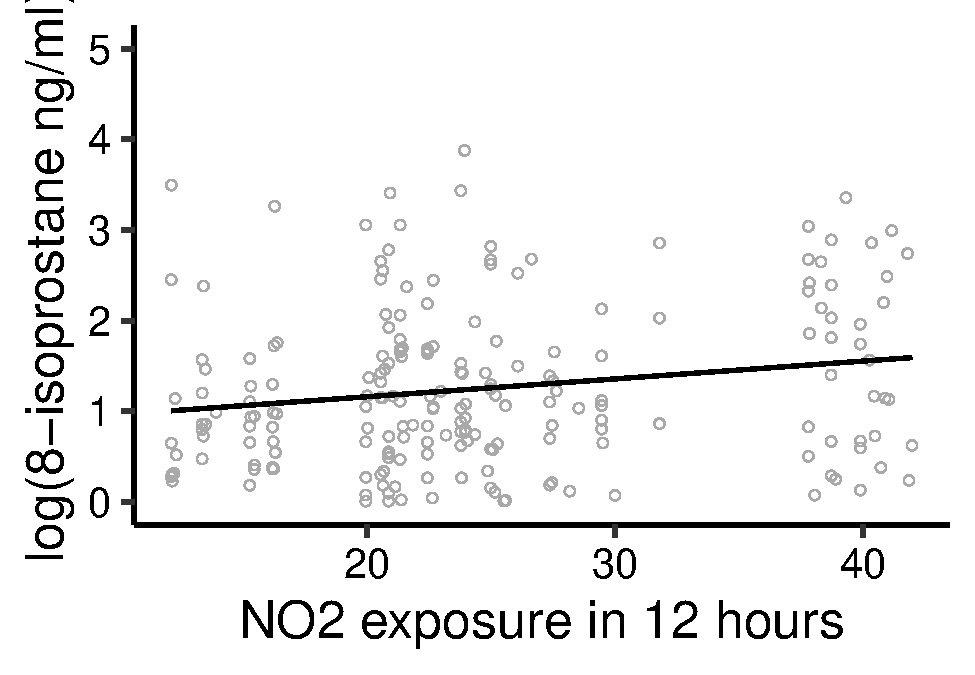
\includegraphics{trial_files/figure-latex/unnamed-chunk-6-1.pdf} Figure
5: Plot of 8-isoprostane

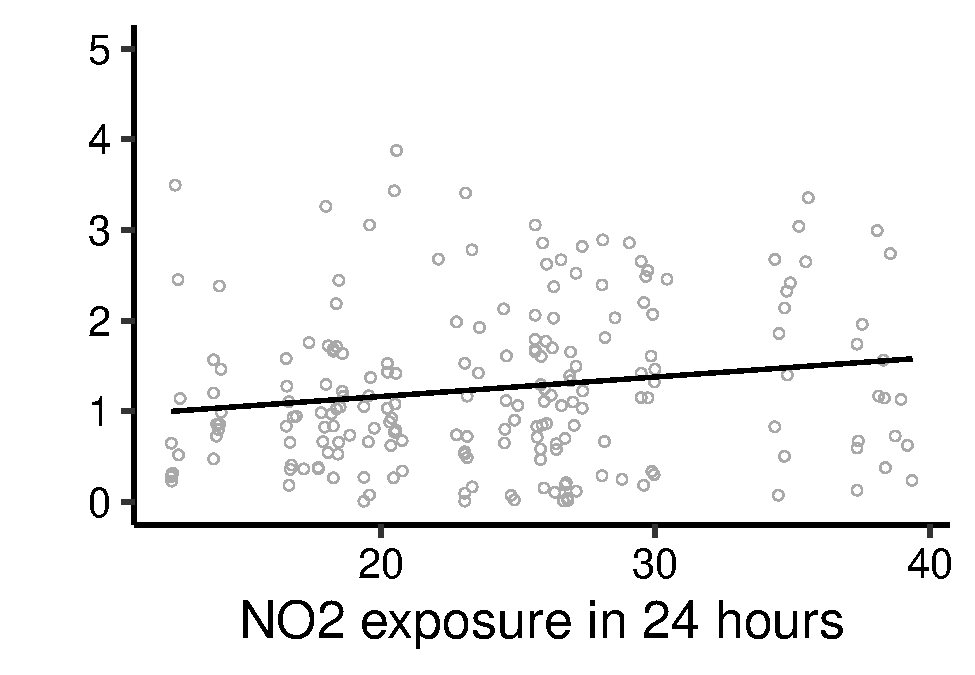
\includegraphics{trial_files/figure-latex/unnamed-chunk-7-1.pdf} Figure
6: Plot of log(8-isoprostane)

\hypertarget{analysis}{%
\section{Analysis}\label{analysis}}

I used linear mixed models with participant-specific intercepts. The
inclusion of participants as a variable in mixed-effects models account
for the correlation of repeated measurements from the same individuals
and precludes the need to control for participant characteristics (e.g.,
age, gender, BMI, the identity of smoker or non-smoker) that do not
change across the four longitudinal measurements.

I used NO2 exposure as predicting variables and log-transformed urinary
biomarkers as dependent variables. For each biomarker, I built 4 models
to the exposure over the periods of 12h, 24h, one week, and two weeks. I
used a backward stepwise model selection method to select the
co-variables for each model. The co-variables that I tested in the
models were last meal, the start of the workday, respiratory infection
status, menstruation, and the time of second-hand exposure. I also
tested the SO2 exposure, ozone exposure and PM2.5 exposure, the average
temperature and humidity during a corresponding period.

With the stepAIC function, the best models were chosen with the lowest
AIC. The vif tests show that there is no model with excess
intercorrelation in the predicting variables. Figure 3 shows that all
four diagnostic plots have the shape of a triangle. The higher the
fitted value is, the higher the residue is. This residue is a result of
skewed distribution of log scaled of the predicting variable .In
general, the residue distribution is not bad. No value is bigger than an
absolute value of 2.5.

Figure 3: diagnostic plots of four final models
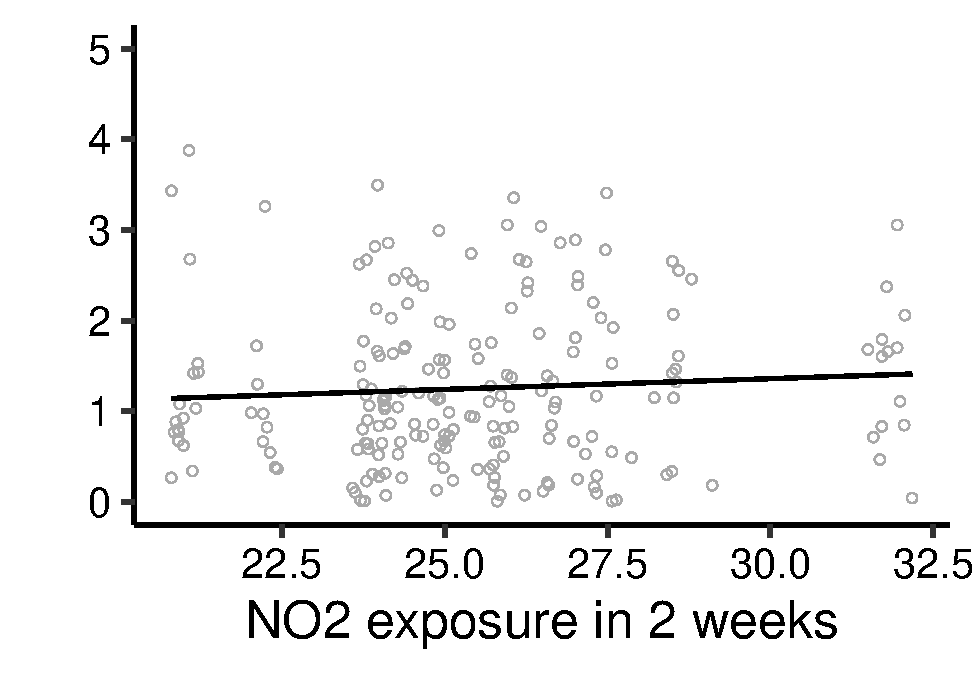
\includegraphics{trial_files/figure-latex/unnamed-chunk-9-1.pdf} Both
12-hour, 24-hour, 1-week and 2-week NO2 exposure showed significant
correlations with the level of urinary 8-isoprostane, especially the
2-week NO2 exposure.

\hypertarget{result-1}{%
\subsection{Result 1}\label{result-1}}

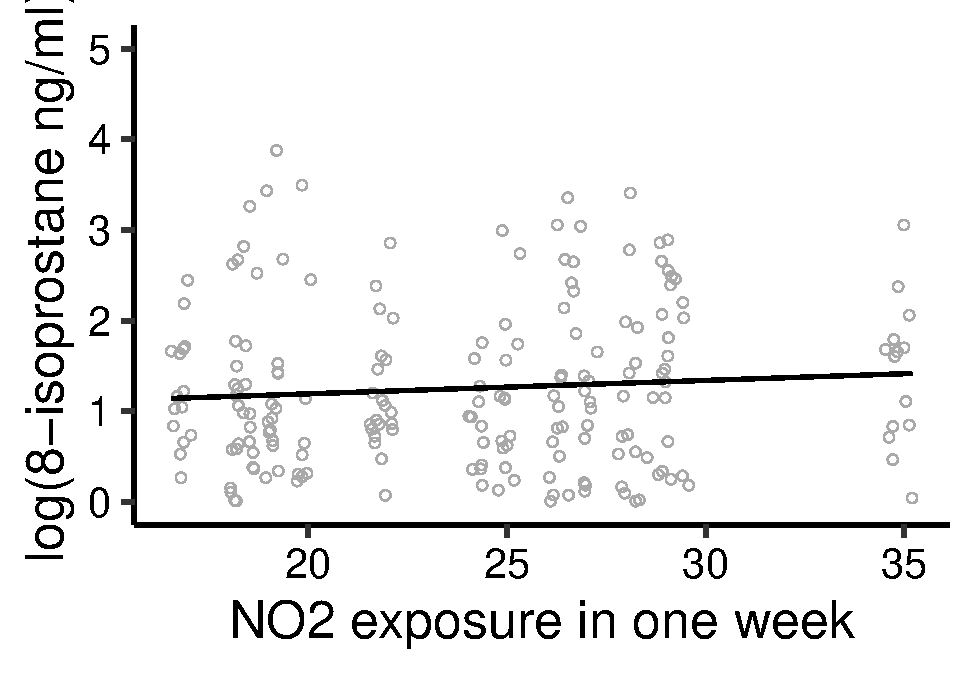
\includegraphics{trial_files/figure-latex/unnamed-chunk-10-1.pdf}


\end{document}
